\documentclass[10pt,a4paper]{article}
\usepackage[latin1]{inputenc}
\usepackage{amsmath}
\usepackage{microtype}
\usepackage[none]{hyphenat}
\usepackage{verbatim}
\usepackage{amsfonts}
\usepackage{amssymb}
\usepackage{enumitem}
\renewcommand{\familydefault}{\sfdefault}
\usepackage{mathpazo}
\renewcommand{\rmdefault}{put}
\usepackage{enumitem}
\usepackage[dvipsnames,svgnames]{xcolor}
\usepackage{tkz-euclide}
\usetkzobj{all}
\usepackage{graphicx}
\usepackage{fancyhdr}
\usepackage{tikz} 	
\usepackage{adjustbox}
\usepackage{pgfplots}
\usepackage{multicol}
\usepackage{lipsum}
\usepackage[left=0.7cm,right=1cm,top=1cm,bottom=1.5cm]{geometry}
\usepackage{cancel} \usepackage{xcolor}
\usepackage{tcolorbox}
\usetikzlibrary{decorations.pathmorphing,patterns}
\usetikzlibrary{decorations.pathreplacing,calc}
 \newcommand\coret[2][red]{\renewcommand\CancelColor{\color{#1}}\cancel{#2}}
\SetLabelAlign{Center}{\hfil\makebox[1.0em]{#1}\hfil}

%%_------= solusi


% Set this =0 to hide, =1 to show

% Set this =0 to hide, =1 to show
\newtcolorbox{mybox}[1][] { colframe = blue!10, colback = blue!3,boxsep=0pt,left=0.2em, coltitle = blue!20!black, title = \textbf{jawab}, #1, } 

%---------- kunci (jika 1 ) muncul
\def\tampilkunci{1}
\newcommand{\hide}[1]{\ifnum\tampilkunci=1
%
\begin{mybox}
 #1
\end{mybox}
%
\vspace{\baselineskip}\fi\ifnum\tampilkunci=0
%
%\vspace{2cm}
%
\fi}



\newcommand*\cicled[1]{\tikz[baseline=(char.base)]{\node[white, shape=circle, fill=red!80,draw,inner sep=0.5pt](char){#1};}}

\newcommand*\kunci[1]{\ifnum\tampilkunci=1
%
\tikz[baseline=(char.base)]{\node[red, shape=circle,draw,inner sep=0.5pt,xshift=2pt](char){#1};}\stepcounter{enumii}
\fi\ifnum\tampilkunci=0
%
\hspace{3pt}#1\stepcounter{enumii}
%
\fi}

\newcommand*\silang[1]{\tikz[baseline=(char.base)]{
\draw[red,thick](-0.2,-0.20)--(0.2,0.2);
\draw[red,thick](-0.2,0.20)--(0.2,-0.2);
\node[black](char){#1};
}}

\newcommand*\centang[1]{\tikz[baseline=(char.base)]{
\draw[red, very thick](-0.2,0.1)--(-0.1,0)--(0.2,0.3);
\node(char){#1};
}}

\newcommand*\merah[1]{
\textcolor{red}{#1}}
\newcommand*\pilgan[1]{
\begin{enumerate}[label=\Alph*., itemsep=0pt,topsep=0pt,leftmargin=*,align=Center] #1 
\end{enumerate}}
\newcommand*\pernyataan[1]{
\begin{enumerate}[label=(\arabic*), itemsep=0pt,topsep=0pt,leftmargin=*] #1 
\end{enumerate}}
\pagestyle{fancy}
\renewcommand{\headrulewidth}{0pt}
\rfoot{\tiny{arifstwan}}
\newcommand{\pilgani}[1]{                            \vspace{-0.3cm}\begin{multicols}{2}
 \begin{enumerate}[label=\Alph*., itemsep=0pt,topsep=0pt,leftmargin=*,align=Center]#1                     \end{enumerate}
 \phantom{ini cuma sapi, wedus, dan ayam}
 \end{multicols}}


\begin{document}


 \textbf{Soal Gelombang Mekanik, berjalan, dan Bunyi} \phantom{ini nama siswa yang aaamengerjakan soal kuis ini }  

No callculator allowed !  
\begin{multicols*}{2}
\begin{enumerate}
% no1 ---------------------------------------------------------
\item Perhatikan peryataan berikut !
\pernyataan{
	\item Membutuhkan medium untuk merambat
	\item Berhubungan dengan medan magnet yang ditimbulkan listrik
	\item Pasti bisa dirasakan dengan indra peraba
	\item Merupakan gelombang transversal
}
Pernyataan yang merupakan ciri gelombang elektromagnetik adalah . . . .
\pilgani{
	\item 1,2,3
	\item 1,3
	\item[\kunci{C.}] 2,4
	\item 4 saja
	\item semua benar}
\hide{ Gelombang elektromagnetik tidak butuh medium, dan merambat secara transversal. Secara umum, getaran/gelombang yang dapat dirasakan adalah gelombang mekanik, misalnya bunyi, gempa bumi, gelombang air laut, dsb
}

% no1b ---------------------------------------------------------
\item [1.b] Berdasarkan arah getarnya, berikut yang termasuk gelombang longitudinal adalah  . . . . 
\pilgan{
	\item bunyi, cahaya, sinyal radio
	\item radio, sinar-x, gamma
	\item gelombang di dalam air, slinky, radio
	\item [\kunci{D.}] gelombang di dalam air, bunyi, slinky
	\item gelombang permukaan air, radio, slinky 
	}
\hide{
baca jenis-jenis gelombang. Hint : gelombang elektromagnetik semuanya dianggap transversal !
}


% no2 ---------------------------------------------------------
\item Dua buah gelombang koheren merambat dan melewati suatu titik. Maka sifat yang terjadi pada titik tersebut adalah . . . 
\pilgan{
	\item Amplitudo jadi dua kali semula
	\item Amplitudo adalah $A_1$ ditambah $A_2$
	\item[\kunci{C.}] frekuensi di titik tersebut sama dengan asal
	\item frekuensi menjadi dua kali frekuensi asal
	\item periode jadi dua kalinya}
\hide{
Koheren artinya mereka beda fasenya sama terus. Artinya frekuensinya sama. Interferensi tidak selalu maksimal (dijumlah). Interferensi maksimal jika mereka fasenya sama $\phi$ = 0 atau $\phi$ = 1. Namun akan minimal jika beda fasenya $\phi = \frac{1}{2}$ 

}


% no2b ---------------------------------------------------------
\item [2.b] Pernyataan yang benar mengenai interferensi dua gelombang pada suatu titik adalah . . . . 
\pilgan{
	\item Amplitudo menjadi dua kali jika beda sudut fase $\pi$
	\item Destruktif jika beda sudutnya $2\pi$
	\item [\kunci{C.}] Konstruktif jika beda sudutnya $2\pi$
	\item Akan melemah jika sefase atau beda fase 1
	\item  Tidak berpengaruh }
\hide{ Pembahasan pada soal sebelumnya }


% no3 ---------------------------------------------------------
\item Perhatikan pernyataan berikut!
\pernyataan{
	\item bisa dipantulkan
	\item bisa mengalami interferensi
	\item mengalami pembiasan
	\item mengalami polarisasi
	}
Dari pernyataan di atas, sifat-sifat gelombang yang menunjukkan karakter gelombang bunyi adalah . . . 
\pilgani{
	\item [\kunci{A.}]1, 2, 3
	\item 1, 3
	\item 2, 4
	\item 4 saja
	\item semua benar}
\hide{Gelombang bunyi adalah gelombang longitudinal. Gelombang longitudinal memiliki pembeda dengan transversal, yakni \textbf{tidak bisa } mengalami \textbf{polarisasi}. Sifat gelombang lainnya ikut mengalami
}


% no4 ---------------------------------------------------------

\item Pernyataan yang benar tentang gelombang riak air adalah . . .
\pilgani{
        \item gel transversal
        \item[\kunci{B.}] gel longitudinal
        \item tidak dapat terinterferensi
        \item tidak dapat dipantulkan
        \item energi tidak mengalir
        }
     
\hide{ Perhatikan riak air di permukaan. Bentuk gelombangnya adalah transversal dan mengalami semua sifat-sifat gelombang.  }


% no5 ---------------------------------------------------------
\item Perhatikan pernyataan berikut!
\pernyataan{
  \item Merupakan gelombang transversal
  \item Merupakan gelombang longitudinal
  \item Dapat di polarisasi
  \item dapat mengalami refleksi}
Pernyataan yang benar mengenai gelombang bunyi adalah . .. 
\pilgani{
        \item 1,3
        \item [\kunci{B.}]2,4
        \item 1,2, dan 3
        \item 4 saja
        \item semua benar
        }
\hide{ Gelombang bunyi longitudinal dan tidak bisa dipolarisasi. Pilihannya sangat jelas hanya 2 dan 4 }

  


% no6 ---------------------------------------------------------
\item Suatu gelombang merambat dengan kecepatan 40 m/s. Gabus pada permukaan gelombang air laut naik turun sebanyak 4 kali tiap detik. Maka panjang gelombang air laut tersebut adalah . . . 
\pilgani{
        \item[\kunci{A.}] 10 m
        \item 16 m
        \item 160 m
        \item 200 m
        \item 45 m
        }
\hide{
Naik turun 4 kali adalah $n$, waktunya adalah 4 detik. Maka frekuensi $f=\frac{n}{t} = 4$. Panjang elombang digunakan rumus 

\begin{align*}
v &= \lambda .f\\
40 &= \lambda . 4\\
\lambda &= 10 \text{ m}
\end{align*}

}




% no7 ---------------------------------------------------------
\item Perhatikan hubungan pada pembiasan berikut
\begin{align*}
n_1.v_1 &=n_2.v_2 \\
n_1.\lambda_1.\coret{f} &= n_2.\lambda_2.\coret{f}\\
\phantom{a}\\
n &\text{ adalah indeks bias pada medium}
\end{align*}
Panjang gelombang di medium dengan indeks bas 1,5 adalah 40cm. Maka panjang gelombang di medium yang memiliki indeks bias 1,2 adalah . .
\pilgani{
    \item[\kunci{A.}] 50 cm
    \item 40 cm
    \item 30 cm
    \item 20 cm
    \item 10 cm}

 \hide{
    Panjang gelombang dan indeks bias berbanding terbalik
    \begin{align*}
    \lambda_1.n_1 &=\lambda_2.n_2\\
    40cm.1,5 &= \lambda_2.1,2\\
    \lambda_2 &= 50 cm\\
    \end{align*}
 }




% no8 ---------------------------------------------------------
\item Pada sebuah gelombang memiliki kecepatan 20 m/s. Jika frekuensinya adalah 4 Hz, maka panjang gelombangnya adalah . . .
\pilgani{
        \item 20 m
        \item [\kunci{B.}]5 m
        \item 4 m
        \item 2 m
        \item 0,5 m
        }
\hide{gunakan $v =\lambda.f$ }



% no9 ---------------------------------------------------------
\item Pasangan panjang gelombang dan frekuensi yang menghasilkan kecepatan 200 m/s adalah . . .
\pilgani{
        \item 2 m dan  400 Hz
        \item 1 m dan 100 Hz
        \item [\kunci{C.}] 2 m dan 100 Hz
        \item 2 m dan 200 Hz
        \item 1 m dan 50 Hz
        }
\hide{gunakan $v =\lambda.f$ }






% no10 ---------------------------------------------------------
\item  Gelombang longitudinal dengan jarak antara regangan dan regangan lagi adalah 2 m. Jika kecepatan rambat adalah 100 m/s, maka frekuensinya adalah . . . 
\pilgani{
        \item [\kunci{A.}] 50 Hz
        \item 100 Hz
        \item 200 Hz
        \item 400 Hz
        \item 600 Hz
        }
\hide{Jarak regangan ke regangan bisa digambar sebagai lembah ke lembah. (gambar sendiri)

Sehingga dipastikan jarak 2m adalah 1 $\lambda$.
\begin{align*}
v&=\lambda.f\\
100&= 2.f\\
f&=50 Hz
\end{align*}

}





% no11 ---------------------------------------------------------
\item


% no12 ---------------------------------------------------------
\item


% no13 ---------------------------------------------------------
\item



% no14 ---------------------------------------------------------
\item 



% no15 ---------------------------------------------------------
\item Suatu gelombang memiliki persamaan $y = 3 \sin (4\pi t - 0,5\pi x)$, dengan satuan sekon dan meter. Maka panjang gelombang kecepatan rambat gelombang adalah . . . .
\pilgani{
    \item 2 m dan 2 m/s
    \item 4 m dan 3 m/s
    \item 2 m dan 3,5 m/s
    \item [\kunci{D.}] 4 m dan  8 m/s
    \item 4 m dan 12 m/s}
\hide{
    \begin{align*}
    v &=\frac{\omega}{k}\\
    v &=\frac{4\pi}{0,5\pi} = 8\text{ m/s}\\
    \phantom{a}
    \frac{2\pi}{\lambda}&= k\\
    \frac{2\pi}{\lambda} &=0.5\pi\\
    \lambda &= 4 \text{ m}
    \end{align*}
}

% no16  ---------------------------------------------------------
\item




% no17  ---------------------------------------------------------
\item




% no18  ---------------------------------------------------------
\item  



% no19  ---------------------------------------------------------
\item Perhatikan gambar gelombang berikut!

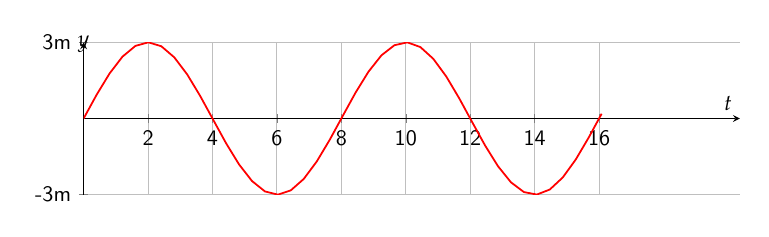
\begin{tikzpicture}[scale=0.8]
\begin{axis}[
   axis x line=center,
   ylabel={$y$},
   xlabel={$t$}, 
   axis y line=middle,
   every axis y label/.style={at={(current axis.north west)},above=2mm}, 
   xtick={0,1.5708,3.14159,...,14},
   xticklabels={0,2,...,16},
   ytick={-1,0,1},
   yticklabels={-3m, 0, 3m},
   xmin=.0, xmax=16,
   domain=0:4.02*pi, width=12cm,height=4cm,
   samples=41,grid]
  \addplot[thick, red, no marks] {sin(deg(x))};
  \end{axis}
  \end{tikzpicture}
  
  Jika panjang tali di atas adalah 8 m, maka persamaan gelombang yang tepat adalah . . .
   \pilgan{
     \item[\kunci{A.}] $y=3 \sin(0,25\pi t -0,5\pi x)$
     \item $y=6 \sin(0,25\pi t -0,5\pi x)$ 
     \item $y=3 \sin(0,5\pi t -0,5\pi x)$
     \item $y=6 \sin(0,5\pi t -0,25\pi x)$
     \item $y=3 \sin(0,25\pi t -0,25\pi x)$
}
\hide{
    Pesamaan gelombang $y=A sin (\omega t - kx)$ maka 
    \begin{align*}
    f &= \frac{n}{t} =\frac{2}{16}=\frac{1}{8}\\
    2\lambda &= 8 m\\
    \lambda &= 4 m\\
    \phantom{a}\\
    y  &= 3 \sin(2\pi\frac{1}{8} t - \frac{2\pi}{4}x)\\
    y &= 3 \sin(0,25\pi t - 0,5 \pi x)
    \end{align*}
}




% no20  ---------------------------------------------------------
\item Perhatikan gambar gelombang berikut!

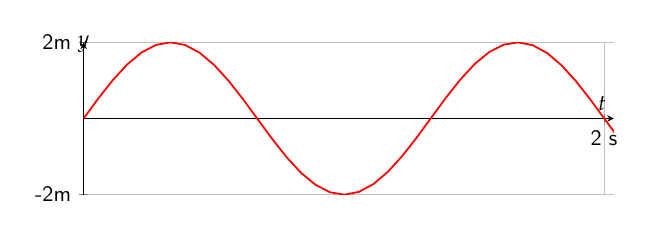
\begin{tikzpicture}[scale=0.8]
\begin{axis}[
   axis x line=center,
   ylabel={$y$},
   xlabel={$t$}, 
   axis y line=middle,
   every axis y label/.style={at={(current axis.north west)},above=2mm}, 
   xtick={0,9.42 },
   xticklabels={0,{2 s}},
   ytick={-1,0,1},
   yticklabels={-2m, 0,2m},
   xmin=.0, xmax=9.6,
   domain=0:3.34*pi, width=10cm,height=4cm,
   samples=41,grid]
  \addplot[thick, red, no marks] {sin(deg(x))};
  \end{axis}
  \end{tikzpicture}
  
  Jika panjang tali di atas adalah 12 m, maka persamaan gelombang yang tepat adalah . . .
   \pilgan{
         \item $y=4 \sin(0,25\pi t -0,5\pi x)$ 
      \item[\kunci{B.}] $y=2 \sin(1,5\pi t -0,25\pi x)$
     \item $y=4 \sin(0,5\pi t -0,5\pi x)$
     \item $y=2 \sin(0,5\pi t -0,25\pi x)$
     \item $y=2 \sin(0,25\pi t -0,25\pi x)$
}
\hide{
Gunakan cara seperti gambar sebelumnya  
}




% no21  ---------------------------------------------------------
\item Suatu gelombang memiliki persamaan $y=4 \sin(0,2\pi x) \cos (3\pi t)$, panjang gelombang dan jenis gelombangnya adalah . . .
\pilgan{
	\item 4 m dan stasioner ujung bebas
	\item[\kunci{B.}] 10 m dan stasioner ujung terikat
	\item 10m dan stasioner ujung bebas
	\item 4 m dan stasioner ujung terikat
	\item 4 m dan berjalan }
\hide{
Aturan sederhana

jika $x$ dalam aturan sinus maka ujung terikat 

jika $x$ dalam aturan cos maka ujung bebas

Pada soal $\sin(0,2\pi x)$, maka ujung terikat. Mencari panjang gelombang dengan
\begin{align*}
k&= \frac{2 \pi}{\lambda}\\
0,2 \pi &= \frac{2\pi}{\lambda}\\
\lambda &= 10 \text { m}
\end{align*}

}





% no22  ---------------------------------------------------------
\item Suatu gelombang memiliki persamaan $y=4 \sin(0,2\pi x) \cos (4\pi t)$, kecepatan rambat gelombang adalah . . . 
\pilgani{
	\item 2 m/s
	\item 0,5 m/s
	\item 0,4 m/s
	\item [\kunci{D.}] 20 m/s
	\item 10 m/s
	}
\hide{kecepatan pada persamaan gelombang bisa dikerjakan dengan menggunakan $\omega$ dan $k$ secara langsung
\begin{align*}
v&=\frac{\omega}{k}\\
v &= \frac{4\coret{\pi}}{0,2\coret{\pi}}\
v & = 20 \text{ m/s}
\end{align*}

}





% no23  ---------------------------------------------------------
\item  Persamaan gelombang adalah $y=4 \cos (2\pi t) \sin( 0,1 \pi x)$. Jarak simpul ke-3 dari ujung getar adalah . . .
\pilgani{
        \item 4 m
        \item 0,1 m
        \item 0,5 m
        \item 10 m
        \item 20 m }
\hide{ Berdasarkan aturan sebelumnya, ini adalah gelombang ujung terikat. tentukan $\lambda$
\begin{align*}
k &=\frac{2\pi}{\lambda}\\
0,1\pi & = \frac{2\pi}{\lambda}\\
\lambda &= 20 \text{ m}
\end{align*}

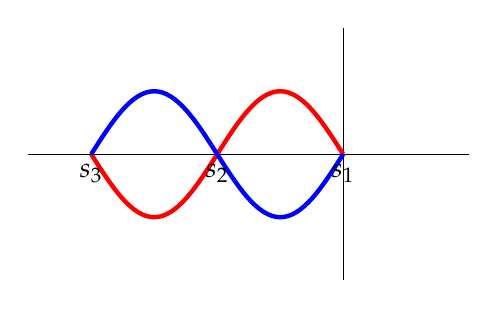
\begin{tikzpicture}[scale=0.8]
\draw(-5,0) -- (2,0) ;
\draw(0,-2)--(0,2);
\draw[ultra thick, red] (0,0) sin (-1,1) cos (-2,0) sin (-3,-1) cos (-4,0);
\draw[ultra thick, blue] (0,0) sin (-1,-1) cos (-2,0) sin (-3,1) cos (-4,0);
\foreach \x/\y in {0/{$s_1$},-2/{$s_2$},-4/{$s_3$}}{
\node at (\x,-0.3cm){\y};}
\end{tikzpicture}

Karena $s_3$ jaraknya adalah 1 gelombang, maka $s_3$= 20 m}

% no24  ---------------------------------------------------------
\item Persamaan getar suatu gelombang adalah $y=8\sin(8\pi t) \cos (0,4 \pi x ) $. Jarak simpul pertama dan perut ketiga adalah . . .
\pilgani{
        \item [\kunci{A.}]$\frac{15}{4}$ m 
        \item 2 m
        \item 5 m 
        \item 8 m 
        \item 10 m 
        }
\hide { Gambar dulu seperti gambar di atas. Karena $\cos(kx)$ maka ujung bebas

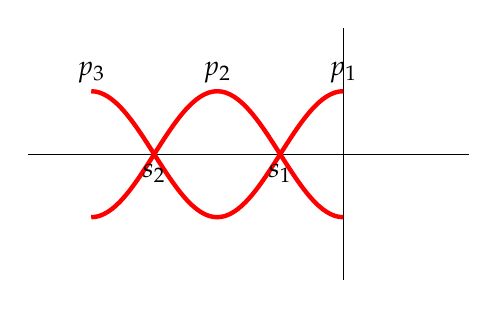
\begin{tikzpicture}[scale=0.8]
\draw(-5,0) -- (2,0) ;
\draw(0,-2)--(0,2);
\draw[ultra thick, red] (0,1) cos (-1,0) sin (-2,-1) cos (-3,0) sin (-4,1);
\draw[ultra thick, red] (0,-1) cos (-1,0) sin (-2,1) cos (-3,0) sin (-4,-1);

\foreach \x/\y in {0/{$p_1$},-2/{$p_2$},-4/{$p_3$}}{
\node at (\x,1.3cm){\y};}

\foreach \x/\y in {-1/{$s_1$},-3/{$s_2$}}{
\node at (\x,-0.3cm){\y};}

\end{tikzpicture}

Jarak $s_1$ ke $p_3$ adalah $\frac{3}{4} \lambda$ maka $s=\frac{3}{4}\times 5=\frac{15}{4}$ m



}



% no25  ---------------------------------------------------------
\item Persamaan getar suatu gelombang adalah $y=8\sin(8\pi t) \cos (0,4 \pi x ) $. Periode gelombang tersebut adalah . . .
\pilgani{
        \item 4 s
        \item[\kunci{B.}] 0,25 s
        \item 0,5 s
        \item 1 s
        \item 2 s
        }
\hide { $\omega = 2\pi f$ maka frekuensi adalah 4 Hz. Sehingga periodenya 1/$f$ = 0,25 s }




% no26  ---------------------------------------------------------
\item Persamaan getar suatu gelombang adalah $y=8\sin(8\pi t) \cos (0,4 \pi x ) $. Kecepatan rambat gelombang tersebut adalah . . .
\pilgani{
        \item [\kunci{A.}] 20 m/s
        \item 40 m/s
        \item 50 m/s
        \item 80 m/s
        \item 10 m/s
        }
\hide{Kecepatan rambat 
\begin{align*}
v&=\frac{\omega}{k}\\
v&=\frac{8\pi}{0,4\pi}\\
v&=20 \text{ m/s}
\end{align*}}



% no27  ---------------------------------------------------------
\item Suatu gelombang dengan persamaan $y=4\sin(4\pi t) \cos (0,5\pi x)$. Jarak simpul ketiga dari titik pantul . . . .
\pilgani{
        \item 2 m
        \item 3 m
        \item 5/4 m
        \item 4 m
        \item [\kunci{E.}]5 m}

\hide{ silakan gambar seperti yang sebelumnya}


% no28  ---------------------------------------------------------
\item Suatu gelombang dengan persamaan $y=4\sin(4\pi t) \cos (0,5\pi x)$. Jarak perut ke 1 dari titik pantul adalah . . .
\pilgani{ 
        \item [\kunci{A.}] 0 m
        \item 5/4 m
        \item 4 m
        \item 5 m
        \item 3 m
        }
\hide{ silakan gambar seperti yang sebelumnya}






% no29  ---------------------------------------------------------
\item Suatu gelombang dengan persamaan $y=4\sin(4\pi t) \cos (0,5\pi x)$. Amplitudo sumber gelombang adalah . . . . 
\pilgani{
        \item 1 m
        \item[\kunci{B.}] 2 m
        \item 3 m
        \item 4 m
        \item tidak ada
        }
\hide{ silakan gambar seperti yang sebelumnya}






% no30  ---------------------------------------------------------
\item Suatu gelombang dengan persamaan $y=4\sin(4\pi t) \cos (0,5\pi x)$. Simpangan di titik dengan jarak 2/3 m pada saat $t=\frac{1}{12}$ s adalah . . .
\pilgani{
        \item[\kunci{A.}] $\sqrt{3}$
        \item 2 $\sqrt{3}$
        \item 2 
        \item 4
        \item 2 $\sqrt{2}$}

\hide{masukan nilai $t$ dan $x$ dalam persamaan, sehingga
\begin{align*}
y&=4\sin(4\pi t) \cos (0,5\pi x)\\
y&=4\sin(4\pi \frac{1}{12})\cos(0,5\pi \frac{2}{3})\\
y&= 4 \sin(\frac{\pi}{3})\cos(\frac{\pi}{3})\\
y&=4.\frac{1}{2}\sqrt{3}\frac{1}{2}\\
y&=\sqrt{3}
\end{align*}
}







% no31 ---------------------------------------------------------
\item Pengaruh memperbesar amplitudo terhadap bunyi adalah . . . 
\pilgani{
	\item [\kunci{A.}] Suara semakin keras (volume)
	\item Frekuensi makin tinggi
	\item frekuensi rendah
	\item taraf intensitas semakin rendah
	\item butuh energi lebih rendah}
\hide{ Amplitudo membutuhkan energi lebih tinggi, selain itu semakin besar amplitudo suara semakin keras (intensitas semakin tinggi) }

% no31.b ----------------------------------------------------------
\item[31.b] Pengaruh frekuensi bunyi yang semakin tinggi adalah . . . (hint: $v=\lambda . f$)
\pilgani{
	\item kecepatan semakin besar
	\item panjang gelombang makin besar
	\item[\kunci{C.}] panjang gelombang makin pendek
	\item suara makin kuat (keras) 
	\item taraf intensitas makin besar
}
\hide{Kecepatan bunyi pada suatu keadaan (misal di medium udara) akan tetap selama faktor2 tetap. Faktor tersebut misalnya (gaya pada tali, massa jenis tali, massa jenis medium, dsb). 

Jadi saat frekuensi naik panjang gelombangnya yang semaki kecil}

% no31.c ---------------------------------------------------------------------

% no32 ---------------------------------------------------------
\item Kuningan memiliki massa jennis 8400 kg/m$^3$. Pada suatu kabel dengan bahan kuningan dan memiliki modulus elastisitas sebesar 2,1 x  10$^9$ N/m$^2$, maka kecepatan suara pada kuningan tersebut adalah . .. 
\pilgani{
	\item 300 m/s
	\item 250 m/s
	\item[\kunci{C.}] 500 m/s
	\item 420 m/s
	\item 600 m/s }
\hide{ 
\begin{align*}
v&=\sqrt{\frac{E}{\rho}}\\
\phantom{a}\\
E&: \text{ Modulus elastisitas/young}\\
\rho &: \text{ Massa jenis zat}\\
\phantom{a}\\
v &= \sqrt{\frac{2,1\times 10^9}{8400}}\\
v& =\sqrt{250000}=500 \text{ m/s}
\end{align*} }


% no33 ---------------------------------------------------------
\item Perhatikan pernyataan berikut tentang pernyataan melde
\pernyataan{
	\item Memperpanjang tali
	\item mengubah tali dengan massa jenis lebih kecil
	\item mengubah beban dengan yang lebih besar
	\item memendekan talli
	}
Usaha yang dapat dilakukan untuk meningkatkan frekuensi adalah . . . ({ hint: frekuensi sebanding dengan kecepatan})
\pilgani{
	\item 1,3
	\item 1,2,3
	\item [\kunci{C.}]2,3,4
	\item 2,4
	\item 4 saja}
\hide{Lihat rumus pada soal no 34}


% no33.b -------------------------------------------------------
\item Cepat rambat gelombang pada tali dituliskan pada rumus
$$ v = \sqrt{\frac{F.l}{m}} =\sqrt{\frac{F}{\mu}} $$
Suatu tali dengan massa 10 gram dan panjang 2 m digantungi beban dengan massa 800 gram. Maka kecepatan getar pada tali tersebut adalah . . . 
\pilgani{
    \item 10 m/s
    \item 20 m/s
    \item [\kunci{C.}]40 m/s
    \item 50 m/s
    \item 100 m/s}
\hide{
    Pada soal tersebut sudah jelas bahwa kecepatan tinggal masukan pada persamaan, sehingga
    \begin{align*}
    v& =\sqrt{\frac{F.l}{m}}\\
    v&=\sqrt{\frac{8.2}{0,01}}=\sqrt{1600}=40\text{ m/s}
    \end{align*}
}


% no34 ---------------------------------------------------------
\item Pipa organa terbuka dengan panjang tabung 10cm berada pada keadaan nada dasar menghasilkan frekuensi 1650 Hz. Maka kecepatan bunyi pada saat tersebut adalah . . . 
\pilgani{
	\item 300 Hz
	\item 320 Hz
	\item[\kunci{C.}] 330 Hz
	\item 340 Hz
	\item 350 Hz
	}
\hide{ nada dasar pipa organa terbuka artinya terbentuk $\frac{1}{2}\lambda$=10 cm, sehingga $\lambda = 20 $ cm. Gunakan rumus umum v dan f
\begin{align*}
v &= \lambda f \\
v &= 0,2 \times 1650 \\
v &= 330 \text{ m/s}
\end{align*}

}


% no34b ---------------------------------------------------------
\item [34.b]  Pada suatu laboraturium kecepatan suara di udara adalah 300 m/s. Jika pipa organa tertutup beresonansi pada nada atas ke 2 dengan frekuensi 1500 Hz, maka panjang pipa organa tersebut adalah . . 
\pilgani{
	\item 10 cm
	\item[\kunci{B.}] 25 cm
	\item 50 cm
	\item 75 cm
	\item 100 cm}
\hide{
Pipa organa tertutup nada atas ke dua berarti terjadi $\frac{5}{4}\lambda=L$. Oleh karena itu, gunakan rumus biasa $v=\lambda.f$ untuk mencari lambda
\begin{align*}
v&=\lambda f\\
300 &= \lambda. 1500 Hz\\
\lambda &=\frac{1}{5} 
\end{align*}

Sehingga panjang pipa adalah $L =\frac{5}{4}\lambda=\frac{5}{4} \frac{1}{5}$=0,25 m   

}


% no35 ---------------------------------------------------------
\item Suatu organa tertutup memiliki nada dasar 100 Hz, maka frekuensi, jumlah simpul dan perut pada nada atas ke 4 adalah . . .
\pilgani{
	\item  400 Hz, 4 simpul, 4 perut
	\item 400 Hz, 4 simpul, 3 perut
	\item 600 Hz, 3 simpul, 2 perut
	\item 700 Hz, 4 simpul, 4 perut
	\item [\kunci{E.}] 900 Hz, 5 simpul, 5 perut
	}
\hide{Digambar saja }


% no36 ---------------------------------------------------------
\item Pipa organa memiliki resonansi yang berturut-turut dengan frekuensi 480 Hz, 800 Hz, dan 1.120 Hz. Tentukan jenis pipa organa dan nada dasarnya . . . . 
\pilgan{
	\item [\kunci{A.}] tertutup, $f_o$ = 160 Hz
	\item tidak dapat ditentukan,  $f_o$ = 160 Hz
	\item terbuka,  $f_o$ = 200 Hz
	\item terbuka,  $f_o$ = 160 Hz
	\item tertutup,  $f_o$ = 200 Hz }
	
\hide{Pehatikan perbandingannya menggunakan FPB

480 : 800 : 1.120 

3  :  5  :  7

Sehingga dipastikan adalah pipa organa terutup. Nada dasar ada di perbandingan 1 

$f_o=\frac{1}{3} \times 480 = 160 Hz$}


% no36b ---------------------------------------------------------
\item[36.b]  Nada atas pertama pipa organa terbuka dengan panjang 60 cm memiliki mengalami resonansi dengan pipa organa tertutup dan menghasilkan tiga simpul. Maka panjang pipa organa tertutup tersebut adalah . . .
\pilgani{
	\item  [\kunci{A.}] 75 cm
	\item 60 cm
	\item 50 cm
	\item 40 cm
	\item 30 cm
}

\hide{
Resonansi artinya \textbf{frekuensi sama}

Pada nada atas pertama organa terbuka terjadi $\lambda = L = 60cm$, sedangkan pipa organa tertutup tiga simpul adalah ada atas ke dua (silakan gambar) $\frac{5}{4} \lambda = L_2$. Kedua pipa berada pada lingkungan yang sama (kecepatan rambat buni sama)
\begin{align*}
f_1 &= f_2\\
\frac{\coret{v}}{\lambda_1} &= \frac{\coret{v}}{\lambda_2}\\
\lambda_2 &= 60 cm\\
\phantom{a}\\
\text{jadi } & \text{ panjang gelombang tertutup adalah} \lambda_2=60 \text{ cm}\\
\end{align*}
Maka panjang pipa dapat diperoleh dengan $\frac{5}{2}\lambda_2 = L =\frac{5}{4} 60= 75$ cm

}

% no37 ---------------------------------------------------------
\item Seorang maling mengejar polisi yang sedang menggunakan mobil patroli dengan kecepatan 10 m/s. Maling tersebut semangat sehingga menekan gas mobil hingga kecepatan 40 m/s. Jika frekuensi sirine mobil patroli adalah 700 Hz, maka frekuensi yang didengar oleh maling adalah . . . . ($v_{\text{bunyi}}$ = 340 m/s)
\pilgani{
	\item 740 Hz
	\item [\kunci{B.}] 760 Hz
	\item 800 Hz
	\item 600 Hz
	\item 400 Hz }
\hide{  
\begin{align*}
f_p&=\frac{340+40}{340+10}700=760\text{ Hz}
\end{align*}

}


% no37b ---------------------------------------------------------
\item [37.b] Suatu ambulan bergerak dengan kecepatan 144 km/jam medekati seseorang yang sedang mengendarai sepeda motor dengan kecepatan 36 km/jam. Ternyata gerakan pengendara dan ambulan saling mendekat (berlawanan). Pada saat itu frekuensi ambulan adalah 600 Hz. Jika kecepatan rambat bunyi di udara adalah 340 m/s, maka frekuensi yang di dengar pengendara adalah . . .
\pilgani{
	\item[\kunci{A.}] 700 Hz
	\item 552,6 Hz
	\item 1151,02 Hz
	\item 400 Hz
	\item 800 Hz
	}
\hide{  
\begin{align*}
f_p&=\frac{340+10}{340-40}600=700\text{ Hz}
\end{align*}
}

% no38 ---------------------------------------------------------
\item Pada jarak 2 meter dari sumber, terdapat intensitas bunyi sebesar 1,6$\times 10^{-8}$ W/m$^2$. Maka intensitas pada jarak 8 m dari sumber bunyi adalah . . . . 
\pilgani{
	\item[\kunci{A.}] 1$\times 10^{-9}$ W/m$^2$
	\item 1,6$\times 10^{-9}$ W/m$^2$
	\item 4$\times 10^{-9}$ W/m$^2$
	\item 8$\times 10^{-9}$ W/m$^2$
	\item 1$\times 10^{-8}$ W/m$^2$}
\hide{
\begin{align*}
\frac{I_2}{I_1} &=\left (\frac{2}{8} \right)^2\\
\frac{I_2}{1,6}\times 10^{-8}&=\frac{1}{16}\\
I_2 &= 1 \times 10^{-9}
\end{align*}

}



% no39 ---------------------------------------------------------
\item Sebuah mesin jahit menghasilkan intensitas $10^{-8}$ W/m$^2$. Jika di suatu tempat terdapat 100 mesin jahit. Maka taraf intensitas mesin jahit di tempat tersebut  adalah . . . . 
\pilgani{
	\item 40 dB
	\item 50 dB
	\item [\kunci{C.}] 60 dB
	\item 70 dB
	\item 80 dB
	}
\hide{ }


% no39b ---------------------------------------------------------
\item[49.b] Sepuluh buah sumber bunyi menghasilkan taraf intensitas 40 dB. Maka jika ada 1000 sumber bunyi, maka taraf intensitasnya menjadi . . . . 
\pilgani{
	\item 40 dB
	\item 50 dB
	\item [\kunci{C.}] 60 dB
	\item 70 dB
	\item 80 dB
	}
\hide{ }

% no40 ---------------------------------------------------------
\item Taraf intensitas bunyi pada titik A dengan jarak 10 m dari sumber adalah 90 db. Maka taraf intesintas di titik B yang jaraknya 100 m dan titik C yang jaraknya 1000 m adalah . . . .
\pilgani{
	\item 80 dB dan 70 dB
	\item[\kunci{B.}] 70 dB dan 50 dB 
	\item 70 dB dan 60 dB
	\item 80 dB dan 60 dB
	\item 60 dB dan 30 dB 
	}
\hide{
}


\end{enumerate}
\end{multicols*} \end{document} 

